\documentclass{article}
\usepackage{amsmath}
\usepackage{graphicx}
\usepackage{float}
\usepackage{tikz}
\usepackage{pgfplots}
\pgfplotsset{compat=1.18}
\usepgfplotslibrary{statistics}
\usepackage{enumerate}

\title{POL 201 / POL 501 - Practice Problem Set Unit II}
\date{}
\author{}

\begin{document}
\maketitle

\section*{Learning Objectives}
\begin{enumerate}
    \item Use scatterplots to describe relationships between two numerical variables, noting the direction, form, and strength of the relationship, and identify any outliers.
    \item Describe the distribution of a numerical variable by its shape, center, and spread, and note any unusual observations.
    \item Understand and calculate measures of center (mean, median, mode) and measures of spread (standard deviation, range, interquartile range).
    \item Identify the shape of a distribution (symmetric, skewed, unimodal, bimodal, etc.).
    \item Use histograms, box plots, and intensity maps to visualize data distributions.
    \item Define and use robust statistics like median and IQR, especially in the presence of skewness and outliers.
    \item Use frequency tables and bar plots for categorical variables.
    \item Use contingency tables and mosaic plots to examine relationships between categorical variables.
    \item Use side-by-side box plots to compare numerical data across categories.
    \item Interpret graphs and describe their significance in the context of political data.
\end{enumerate}

\newpage

\section*{Questions}

\subsection*{Variable Descriptions and Data Summarizing}

\paragraph{1.} \textbf{Campaign Donations}. The table below shows the number of political campaigns run in different cities and the total amount of donations received:
\begin{center}
    \begin{tabular}{|c|c|c|}
    \hline
    City & Number of Campaigns & Total Donations (in million \$) \\
    \hline
    Metropolis & 4 & 180 \\
    Gotham & 3 & 165 \\
    Star City & 5 & 220 \\
    Central City & 2 & 160 \\
    Atlantis & 7 & 250 \\
    \hline
    \end{tabular}
\end{center}

\begin{enumerate}[a)]
    \item Construct a scatterplot of the data. Describe the direction, form, and strength of the relationship between the number of campaigns and total donations.
    \item Calculate the mean total donations and its median, and discuss why the mode is not applicable to this variable. What does the mean tell you about the shape of the donations distribution when compared to the median?
\end{enumerate}


\subsection*{Analyzing Box Plots}
\paragraph{2.} \textbf{Turnout Across Districts}. Given the following data on voter turnout rates (\%) in 10 districts during the last election:
\begin{center}
    \begin{tabular}{|c|c|}
    \hline
    District & Turnout Rate \\
    \hline
    A & 68 \\
    B & 55 \\
    C & 82 \\
    D & 78 \\
    E & 74 \\
    F & 49 \\
    G & 85 \\
    H & 90 \\
    I & 45 \\
    J & 93 \\
    \hline
    \end{tabular}
\end{center}

\begin{enumerate}[a)]
    \item Create a histogram and a box plot of the turnout rates. Describe the shape, center, and spread of the distribution. For the histogram, use 5 bins of equal size going from the minimum and maximum value of the data. Explain your steps in constructing both graphs.
\end{enumerate}

\subsection*{Comparing Data Across Categories}

\paragraph{3.} \textbf{Policy Support and Age Cohorts}. The table below shows the summary statistics for approval ratings of Policy A and Policy B across two different age groups.

\begin{center}
\begin{tabular}{|c|c|c|c|c|c|c|}
\hline
Age Group & Policy & Mean (\%) & Median (\%) & SD (\%) & Q25 (\%) & Q75 (\%) \\
\hline
18-30 & Policy A & 60 & 62 & 5 & 58 & 64 \\
18-30 & Policy B & 70 & 72 & 7 & 67 & 75 \\
\hline
31-45 & Policy A & 65 & 66 & 4 & 63 & 68 \\
31-45 & Policy B & 62 & 63 & 6 & 59 & 66 \\
\hline
\end{tabular}
\end{center}

\begin{enumerate}[a)]
    \item Use the summary statistics provided in the table to construct side-by-side box plots for Policy A and Policy B approval ratings for each age group. Describe the center, shape, and spread for the distribution of each subgroups.
\end{enumerate}

\paragraph{4.} \textbf{Issue Position Strategy}. You are a campaign strategist tasked with advising a candidate on their position regarding a controversial policy. Your team has conducted surveys in two key electoral districts where the race is competitive. The survey results are presented in a table showing the relative frequency distribution of voter support for the policy on a Likert scale from 1 to 5, where 1 indicates strong opposition and 5 indicates strong support.

\begin{center}
\begin{tabular}{|c|c|c|}
\hline Likert Scale & District A (\%) & District B (\%) \\
\hline
1 - Strongly Oppose & 20 & 15 \\
2 - Oppose & 30 & 18 \\
3 - Neutral & 25 & 17 \\
4 - Support & 15 & 15 \\
5 - Strongly Support & 10 & 35 \\
\hline
\end{tabular}
\end{center}

\begin{enumerate}[a)]
    \item Create bar plots of these distributions and describe which district is more likely to support the policy and which is more likely to oppose it.
    \item For each district's distribution of support for the policy, would you say it is symmetrical, positively skewed (right-skewed), or negatively skewed (left-skewed)?
    \item Calculate the weighted average of voter support in each district using the Likert scale values (1 to 5) and the given percentages for each level of support. Discuss what insights might be missed if we only looked at these averages instead of the full distributions.
\end{enumerate}


\paragraph{5.} \textbf{Policy Impact Analysis}.
Assume you are tasked with assessing the impact of a recent policy implemented by the current administration on public presidential approval ratings. You have the following pre- and post-policy implementation approval ratings from a sample of 1,000 citizens:
\begin{center}
    \begin{tabular}{|c|c|c|}
    \hline
    Time of Survey & Mean Approval Rating & Standard Deviation \\
    \hline
    Pre-Policy & 50\% & 10\% \\
    Post-Policy & 60\% & 25\% \\
    \hline
    \end{tabular}
\end{center}

\begin{enumerate}[a)]
    \item The mean approval rating increased from 50\% to 60\% after the policy implementation, but the standard deviation also increased from 10\% to 25\%. Discuss what the increase in standard deviation suggests about public opinion on presidential approval and how it might limit our understanding of the policy's impact on approval ratings.
\end{enumerate}

\paragraph{6.} \textbf{Support for Public Healthcare}. A recent survey on political opinions regarding government spending on healthcare has been conducted in two states. The results are presented below, using a three-point Likert scale where 1 indicates low support, 2 indicates neutral, and 3 indicates high support.

\begin{center}
\begin{tabular}{|c|c|c|}
\hline Opinion (Scale 1-3) & Respondents in State 1 & Respondents in State 2 \\
\hline 1 (Low Support) & 4,000 & 1,500 \\
2 (Neutral) & 2,000 & 7,000 \\
3 (High Support) & 4,000 & 1,500 \\
\hline
\end{tabular}
\end{center}

\begin{enumerate}[a)]
    \item Calculate the mean approval rating for each state using the provided frequencies (use the formula for the weighted average). Looking only at the mean, what we would infer about the citizens' opinions across these states?
    \item Calculate the standard deviation of the approval ratings for each state. What does the standard deviation tell us about the variation in opinions? \footnote{The following is the formula for the weighted SD: $\text{SD} = \sqrt{\frac{\sum_{i=1}^n w_i (x_i - \bar{x})^2}{\sum_{i=1}^n w_i}} $ where ($w_i$) are the weights (number of respondents), ($x_i$) are the support ratings, and ($\bar{x}$) is the weighted mean.}
    \item Create bar plots to visualize the distribution of opinions in both states. Analyze the results, and discuss why it is important to look at the distribution and standard deviation, not just the mean, when analyzing opinions.
    \item In which of the two states citizens are more neutral in their opinions of the policy? Justify your answer.
\end{enumerate}

\paragraph{7.} \textbf{Strategic Reallocation of Agricultural Funds}. The Secretary of Agriculture is currently reassessing the budget allocation of the department in light of critiques from members of Congress, who claim that the average cost of agricultural programs significantly exceeds that of similar federal initiatives. With the average program cost surpassing the national benchmark, the President has decided to implement a strategic fund reallocation. This decision involves redirecting funds from the Department of Agriculture to another subdivision of the state, in order to optimize federal spending without reducing the total government budget.

\begin{enumerate}[a)]
    \item In preparation for this reallocation, the Secretary must select 10 agricultural programs for termination. To effectively reduce the average cost of the remaining programs, should the Secretary close the programs that are the most expensive, the least expensive, or those around the average cost?
    \item Assume that the President is considering splitting some existing programs into multiple programs, instead of moving the funds and terminating programs. Would this strategy be effective for reducing the average cost of the programs in the Department of Agriculture? Please justify your answer appropriately.
\end{enumerate}

\paragraph{8.} \textbf{Standard of Living Across Countries}. In a recent international economic forum, data showed that Country A has a Gross Domestic Product (GDP) of \$1 trillion, while Country B has a GDP of \$3 trillion. One observer comments that ``\emph{since Country B's GDP is three times larger than Country A's, it is clear that the citizens of Country B enjoy a better standard of living}."
\par How could you use the concept of average income per person in the population (GDP per capita) to analyze the standard of living in these countries and potentially disprove the initial claim? Assume some data if necessary to support your explanation.


\subsection*{Interpreting Graphs}
\paragraph{9.} The following graph shows the number of supporters for two policies (Policy X and Policy Y) over six months:

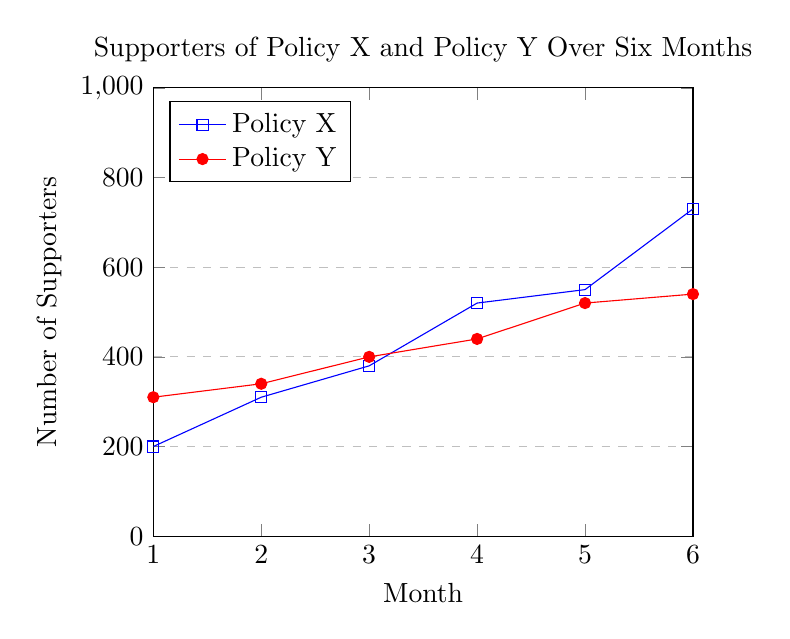
\begin{tikzpicture}
\begin{axis}[
    title={Supporters of Policy X and Policy Y Over Six Months},
    xlabel={Month},
    ylabel={Number of Supporters},
    xmin=1, xmax=6,
    ymin=0, ymax=1000,
    xtick={1,2,3,4,5,6},
    ytick={0,200,400,600,800,1000},
    legend pos=north west,
    ymajorgrids=true,
    grid style=dashed,
]
\addplot[
    color=blue,
    mark=square,
    ]
    coordinates {
    (1,200)(2,310)(3,380)(4,520)(5,550)(6,730)
    };
    \addlegendentry{Policy X}

\addplot[
    color=red,
    mark=*,
    ]
    coordinates {
    (1,310)(2,340)(3,400)(4,440)(5,520)(6,540)
    };
    \addlegendentry{Policy Y}
\end{axis}
\end{tikzpicture}

\begin{enumerate}[a)]
    \item Describe the trend in the number of supporters for Policy X and Policy Y over the six-month period.
    \item Based on the graph, which policy appears to be gaining support more rapidly? Explain your answer.
\end{enumerate}

\paragraph{10.} The following box plot shows the distribution of campaign donations in three cities:

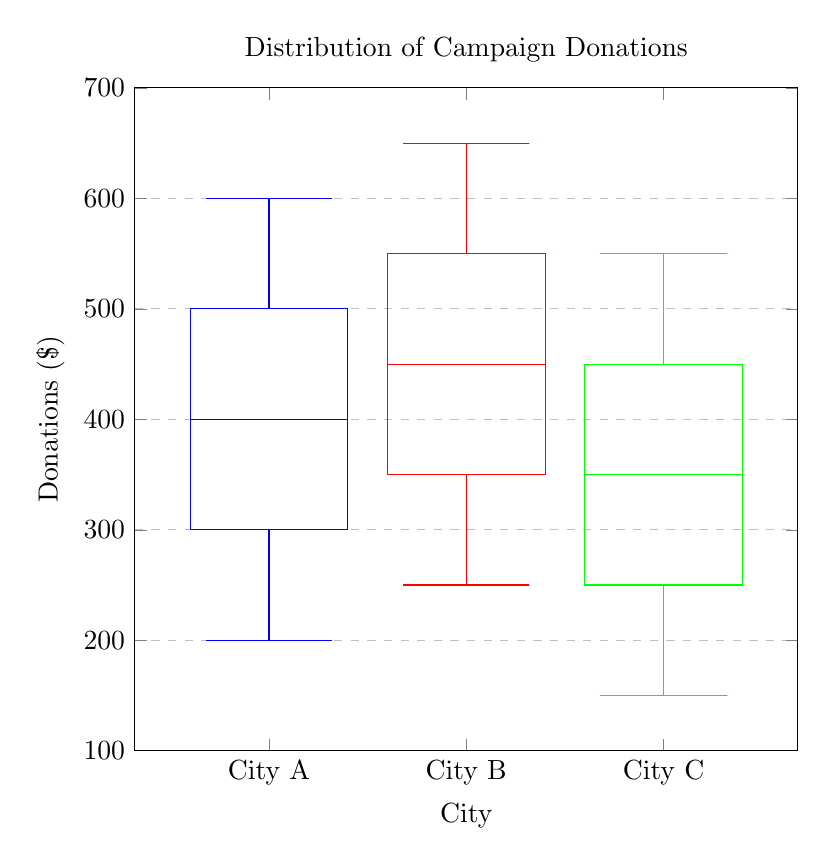
\begin{tikzpicture}
\begin{axis}[
    title={Distribution of Campaign Donations},
    xlabel={City},
    ylabel={Donations (\$)},
    xtick={1,2,3},
    xticklabels={City A, City B, City C},
    ymajorgrids=true,
    grid style=dashed,
    boxplot/draw direction=y,
    width=10cm,
    height=10cm,
    cycle list={{blue},{red},{green}}
]

% Box Plot for City A
\addplot+[
    boxplot prepared={
        median=400,
        upper quartile=500,
        lower quartile=300,
        upper whisker=600,
        lower whisker=200
    },
] coordinates {};

% Box Plot for City B
\addplot+[
    boxplot prepared={
        median=450,
        upper quartile=550,
        lower quartile=350,
        upper whisker=650,
        lower whisker=250
    },
] coordinates {};

% Box Plot for City C
\addplot+[
    boxplot prepared={
        median=350,
        upper quartile=450,
        lower quartile=250,
        upper whisker=550,
        lower whisker=150
    },
] coordinates {};

\end{axis}
\end{tikzpicture}

\begin{enumerate}[a)]
    \item Compare and interpret the median and interquartile range (IQR) of campaign donations across the five cities.
    \item What can you say about the shape of the distribution of donations by looking at the box plots?
\end{enumerate}

\paragraph{11.} The following bar plot shows the number of voters in favor of different policies in a given region:

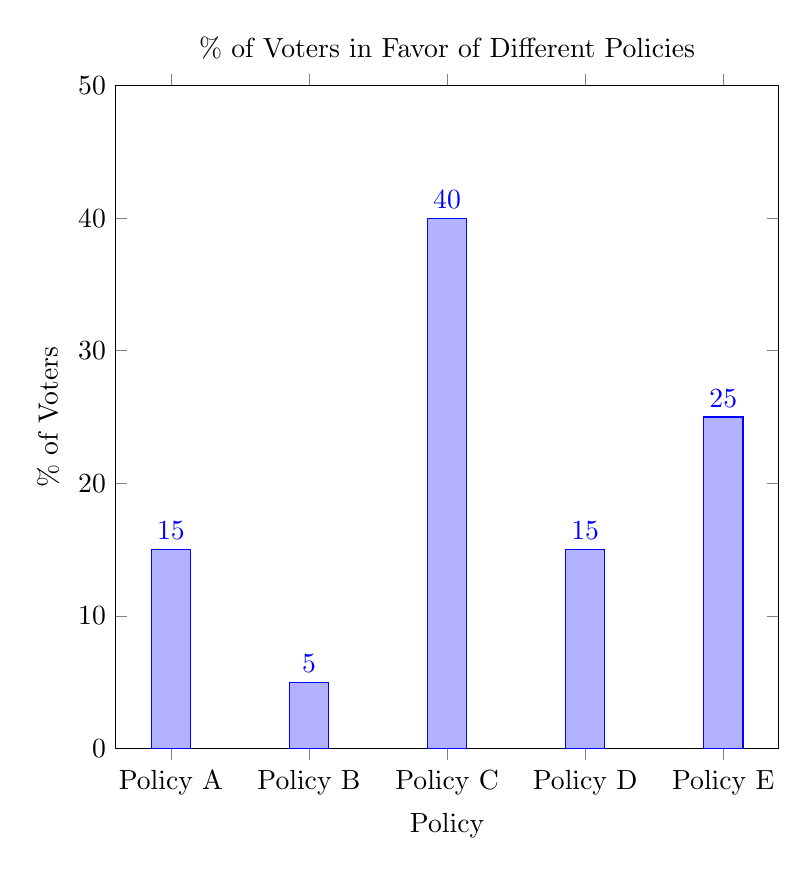
\begin{tikzpicture}
  \begin{axis}[
    title={\% of Voters in Favor of Different Policies},
    xlabel={Policy},
    ylabel={\% of Voters},
    symbolic x coords={Policy A, Policy B, Policy C, Policy D, Policy E},
    xtick=data,
    ybar,
    nodes near coords,
    ymin=0,
    ymax=50,
    width=10cm,
    height=10cm,
    bar width=0.5cm,
    ]
    \addplot coordinates {(Policy A,15) (Policy B,5) (Policy C,40) (Policy D,15) (Policy E,25)};
  \end{axis}
\end{tikzpicture}

\begin{enumerate}[a)]
    \item Describe the distribution of voter support across the different policies.
    \item Which policy has the highest voter support, and which has the lowest?
    \item To better understand the distribution of policy preferences, a friend of yours suggest assigning numbers from 1 to 5 to the policies. Then, calculate the standard deviation to understand the dispersion of preferences. Explain why this would be an incorrect thing to do in this case.
\end{enumerate}

\subsection*{Analyzing Distributions with Similar Central Tendencies}
\paragraph{12.} The table below shows the percentage of voters in two different states expressing their level of support for a new immigration policy on a scale from 1 to 5, with 1 being strongly against the policy and 5 being strongly in favor of the policy:

\begin{center}
    \begin{tabular}{|c|c|c|}
    \hline
    Level of Support & State A (\%) & State B (\%) \\
    \hline
    1 & 13\% & 22\% \\
    2 & 35\% & 18\% \\
    3 & 4\% & 20\% \\
    4 & 35\% & 18\% \\
    5 & 13\% & 22\% \\
    \hline
    \end{tabular}
\end{center}

\begin{enumerate}[a)]
    \item Calculate the mean and median level of support for each state.
    \item Describe the shape of the distribution of support for each state (discuss mode, symmetry, and skewness).
    \item In the context of this question, discuss why it is important to consider the shape of the distribution in addition to the measures of central tendency (mean and median). How does the polarization in State A and the relative uniformity in State B affect the interpretation of the mean and median?
\end{enumerate}

\section*{Glossary - Unit II}

\begin{itemize}
    \item \textbf{Scatterplot}: A graphical representation that displays the relationship between two numerical variables, showing a pattern that may indicate association or independence.
    \item \textbf{Dot plots}: Graphs that display the frequency distribution of individual data points along a number line, useful for visualizing small data sets.
    \item \textbf{Mean}: The average of a data set, calculated by dividing the sum of all values by the number of values.
    \item \textbf{Stacked dot plot}: A variation of dot plots where dots are stacked vertically to better visualize data distribution and frequency.
    \item \textbf{Histograms}: Graphical displays that use bars to show the frequency distribution of a dataset, grouping data into bins or intervals.
    \item \textbf{Bin width}: The range of values in each interval of a histogram, which affects the granularity and interpretation of the data's distribution.
    \item \textbf{Distribution shape}: Characteristics of data distribution including:
    \begin{itemize}
        \item \textbf{Modality}: The number of peaks (unimodal, bimodal, etc.)
        \item \textbf{Skewness}: Symmetry or asymmetry of the data around its central value.
        \item \textbf{Unusual observations}: Notable deviations from other data points, often outliers.
    \end{itemize}
    \item \textbf{Variance}: A measure of data spread calculated as the average squared deviation from the mean, reflecting data variability.
    \item \textbf{Standard deviation}: The square root of variance, providing a measure of dispersion in the same units as the data.
    \item \textbf{Median}: The middle value of a data set when ordered, effectively dividing the dataset into two equal halves.
    \item \textbf{Quartiles and Interquartile Range (IQR)}: Values that divide the data into quarters. The IQR is the range between the first and third quartiles and measures the spread of the middle half of the data.
    \item \textbf{Box plot}: A graphical summary of data showing the median, quartiles, and potential outliers using a box and whiskers format.
    \item \textbf{Robust statistics}: Statistical measures less sensitive to outliers, often preferred in data with unusual observations.
    \item \textbf{Transforming data}: Applying a mathematical function to each data point to change the data's distribution, often to achieve normality or improve symmetry.
    \item \textbf{Intensity maps}: Visual representations that use color to show variations in data across a geographic region.
    \item \textbf{Weighted Mean}: The average of a variable where each value has a specific weight assigned, calculated by multiplying each value by its corresponding weight, summing these products, and then dividing by the sum of the weights.
    \item \textbf{Weighted Standard Deviation}: A measure of the spread of a set of numbers, where each number can have a different level of importance, represented by weights. It is calculated through the following steps:
    \begin{enumerate}
        \item Compute the weighted mean of the data set.
        \item Calculate the squared deviations from the weighted mean for each data point.
        \item Multiply each squared deviation by its corresponding weight.
        \item Sum these weighted squared deviations.
        \item Divide the sum of the weighted squared deviations by the total sum of the weights to obtain the weighted variance.
        \item Take the square root of the weighted variance to get the weighted standard deviation.
    \end{enumerate}
This procedure reflects the varying significance of each data point in the data set.

\end{itemize}

\textbf{Considering categorical data:}
\begin{itemize}
    \item \textbf{Contingency tables}: Tables that summarize the relationship between two categorical variables by displaying frequencies for each combination of categories.
    \item \textbf{Bar plots}: Graphical displays using bars to show frequencies or proportions of categorical data.
    \item \textbf{Mosaic plots}: Plots that visually represent the proportions of categories similar to bar plots but across two or more categories.
    \item \textbf{Pie charts}: Circular charts divided into sectors to show numerical proportions of categories.
\end{itemize}

\textbf{Case study:}
\begin{itemize}
    \item \textbf{Hypothesis testing framework}: A structured approach to determine if observed data can be explained by chance alone or if there are statistically significant differences.
    \item \textbf{Simulating the experiment}: A method to assess the likelihood of the observed outcome under the assumption that the null hypothesis is true.
\end{itemize}


\end{document}
